\section{Blokk rejtjelező módok}

\subsection{Electronic Code Book}

	\begin{center}
		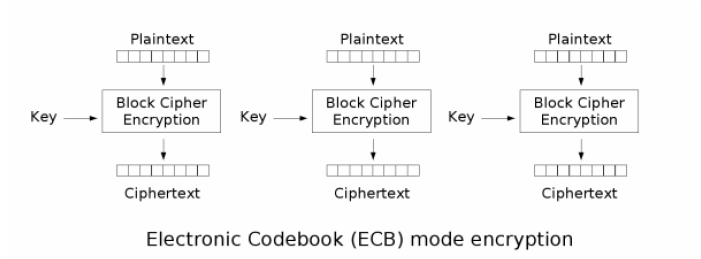
\includegraphics[scale=0.7]{img/ECB}
	\end{center}

	$X_i$ rejtett nyílt blokkot kódoja $E_k$ transzformáció, így kapjuk az elkódolt $Y_i$ üzenetet. $D_K$ dekódoló transzformációval, visszanyerhető az eredeti szöveg
	$$Y_i = E_K(X_i)$$
	$$X_i = D_K(Y_i)$$

\textbf{Biztonság:}
	\begin{itemize}
		\item Kulcs ismerete nélül is törhető: Csinálunk egy szótárat.
		\item Blokkok könnyedén felcserélhetők ( mindig egy blokkot küldjünk és megvan oldva)
	\end{itemize}

\textbf{Hatékonyság:}
	\begin{itemize}
		\item Kódolás, dekódolás sebessége = Blokkrejtjelező sebessége
		\item Tetszőleges sorrendben kódolhatók a blokkok
		\item Adatbázis fájlok rejtjelezésénél használják
	\end{itemize}

\subsection{Cipher Block Chaining}

	\begin{center}
		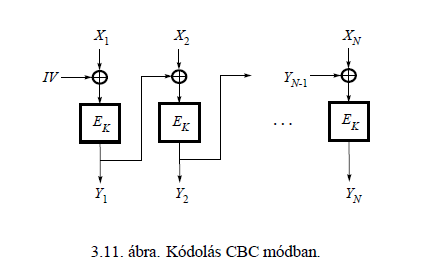
\includegraphics[scale=0.8]{img/CBC}
	\end{center}

\textbf{Kódolás:}

	$$Y_1 = E_K(X_1 \oplus IV) $$
	$$Y_i = E_K(X_i \oplus Y_{i-1})$$

\textbf{Dekódolás: }

	$$X_1 = D_K(Y_1) \oplus IV$$
	$$X_i = D_K(Y_i) \oplus Y_{i-1}$$

$\oplus = xor$, $IV$ = Initial Vector. Kezdeti változó\\[2pt]

\textbf{Hatékonyság:}
	\begin{itemize}
		\item Rejti a szöveg mintáit ( XOR ). Lásd alább a képen
		\item Detektálható a blokkok keveredése, elesztése, helyettesítése, hiszen csak akkor dekódolható , ha pontosan ugyan azt kapja a vevő.
		\item Negatívum, hogyha 2 rejtjeles blokk megegyezik: $Y_i = Y^{,}_j \rightarrow Y_{i-1} \oplus Y^{,}_j = X_i \oplus X^{,}_j.$ De mivel egyenletes eloszlás ennek kicsi az esélye.
	\end{itemize}

\textbf{Hatékonyság:}
	\begin{itemize}
		\item Kódolás, dekódolás sebessége = Blokkrejtjelező sebessége ( XOR elhanyagolható )
		\item Nem párhuzamosítható a kódolás, de dekódolás párhuzamosítható!!
		\item Egy blokk módosítása az összes utána következő módosítását igényli
	\end{itemize}

\begin{center}
\textbf{Összehasonlítás:}
	\begin{center}
		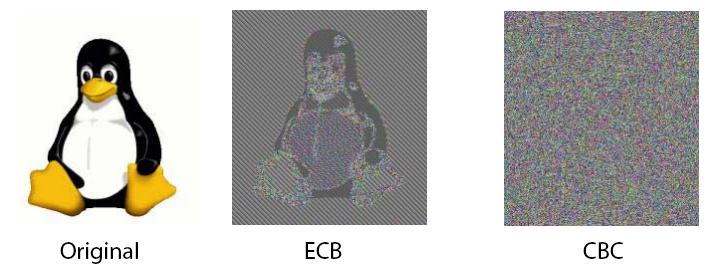
\includegraphics[scale=0.5]{img/ECBCBC}
	\end{center}
\end{center}


\subsection{Cipher FeedBack}

CÉL: Rövid üzenetek, QOS


	\begin{center}
		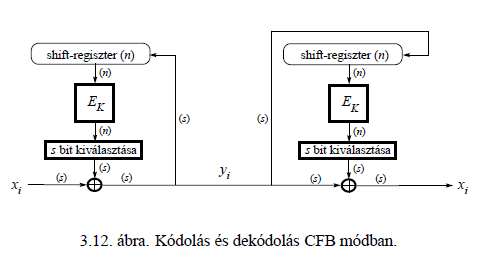
\includegraphics[scale=0.8]{img/CFB}

		\textit{s bites karakter, n bites shift regiszter}
	\end{center}


\textbf{Kódolás:}
	$$Y_1 = X_1 \oplus E_K(IV) $$
	$$Y_i = X_i \oplus E_K(Y_{i-1}) $$

\textbf{Dekódolás:}
	$$X_1 = Y_1 \oplus E_K(IV) $$
	$$X_i = Y_i \oplus E_K(Y_{i-1})$$

\textbf{Hatékonyság:}
	\begin{itemize}
		\item Sebesség $\dfrac{s}{n}$ szerese a blokkrejtjelezőnek. ( $CFB \leq CBC $ )
		\item Ha egy karaktert módosítunk, összes utána lévőt ujra kell dekódolni
		\item Szöveg mintáit elrejti
		\item - Utolsó karakter bitjei manipulálhatók
	\end{itemize}


\subsection{Output FeedBack}

Szinkron kulcsfolyam rejtjelező. CFB től annyiban különbözik ,hogy a rejtjelezett szöveg helyett, a blokkrejtjelező kimenete van hozzákötve.

\begin{center}
	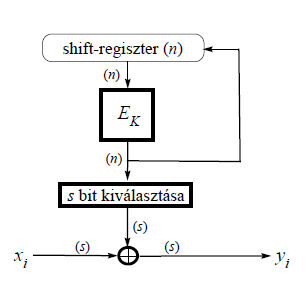
\includegraphics[scale=0.7]{img/OFB}
\end{center}

Itt is kell IV, ehhez általában az üzenet sorszámát használják. (Ha mindig ugyan az lenne az nagy sebezhetőség lenne)

\textbf{Hatékonyság:}
	\begin{itemize}
		\item Sebesség $\dfrac{s}{n}$ szerese a blokkrejtjelezőnek. ( $OFB \leq CBC $ )
		\item - Nem lehet párhuzamosítani
		\item + Offline kiszámolható
		\item + Egy karakter függetlenül változhtatható a többitől
	\end{itemize}

\subsection{CTR - CounTeR}

\begin{center}
	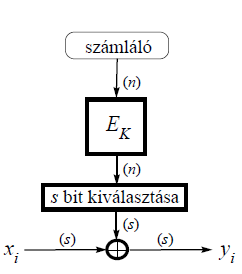
\includegraphics[scale=0.7]{img/CTR}
\end{center}

OFB Módhoz nagyon hasonlít, csak itt nincs visszacsatolás.\\[-2pt]

\textbf{Hatékonyság:}
	\begin{itemize}
		\item + Lehet már párhuzamosítani
		\item Többi tulajdonság megegyezik OFB-vel
	\end{itemize}
